\chapter{Developer documentation}
\label{ch:impl}

This chapter will cover the process of developing a Clang-Tidy checker, and the infrastructure that it is built on.
The developer should have an advanced knowledge of \CC{} and strong typing, minimal user experience with Linux and
Clang-Tidy, and familiarity with declarative programming paradigm.

The work of the thesis and all the code I have written is a contribution and enhancement to the originally existing library
of LLVM Compiler Infrastructure. I have attached the patch file that contains all the modifications to the original code
with the thesis.

\section{Infrastructure}
\label{sec:dev-infra}

The enhancement of the infrastructure focused on implementing the three distinct phases previously discussed in \Cref{ch:user}
for the checkers to distinguish and the developers to use.
\Cref{fig:activity-single} and \cref{fig:activity-multi} demonstrates difference between the old infrastructure
(\texttt{"single"}) and the new one (\texttt{"multi"}).
Note that if the aforementioned compact phase has not been run for a checker, the third phase (diagnose) will perform the "single"
path, as it is the default mode of Clang-Tidy for both backwards compatibility, and intentional usage.

\begin{figure}[H]
	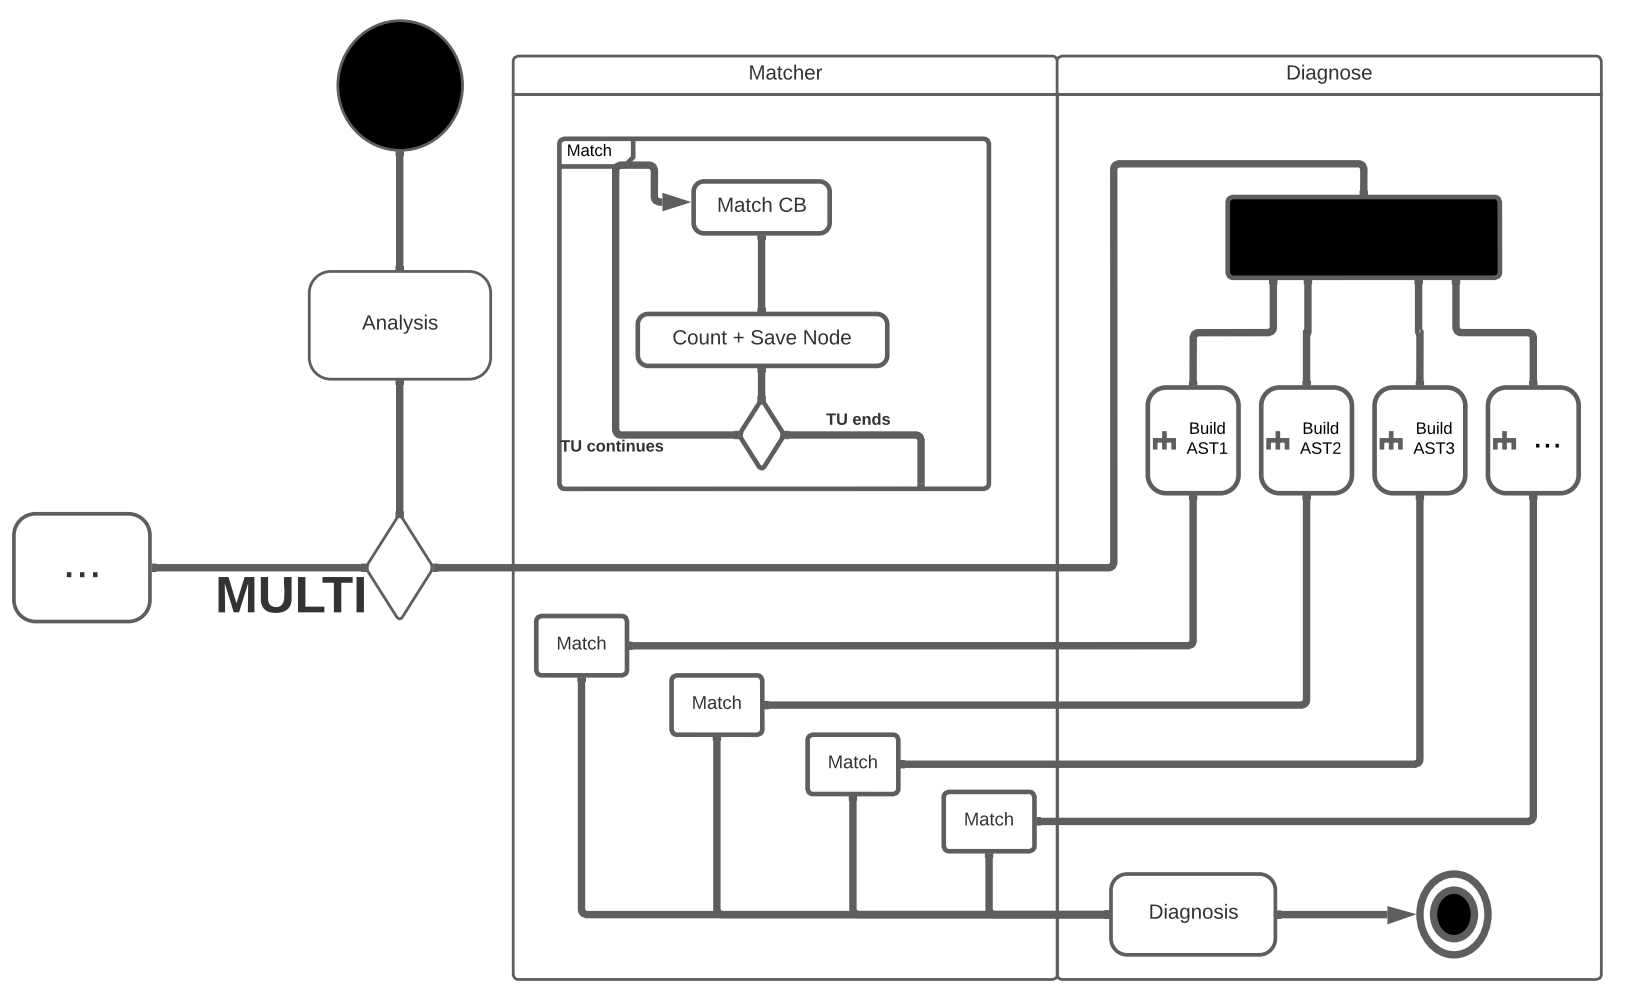
\includegraphics[width=\linewidth]{images/activity_single.png}
	\caption{Activity diagram of Clang-Tidy infrastructure in "single" mode.}
	\label{fig:activity-single}
\end{figure}

\begin{figure}[H]
	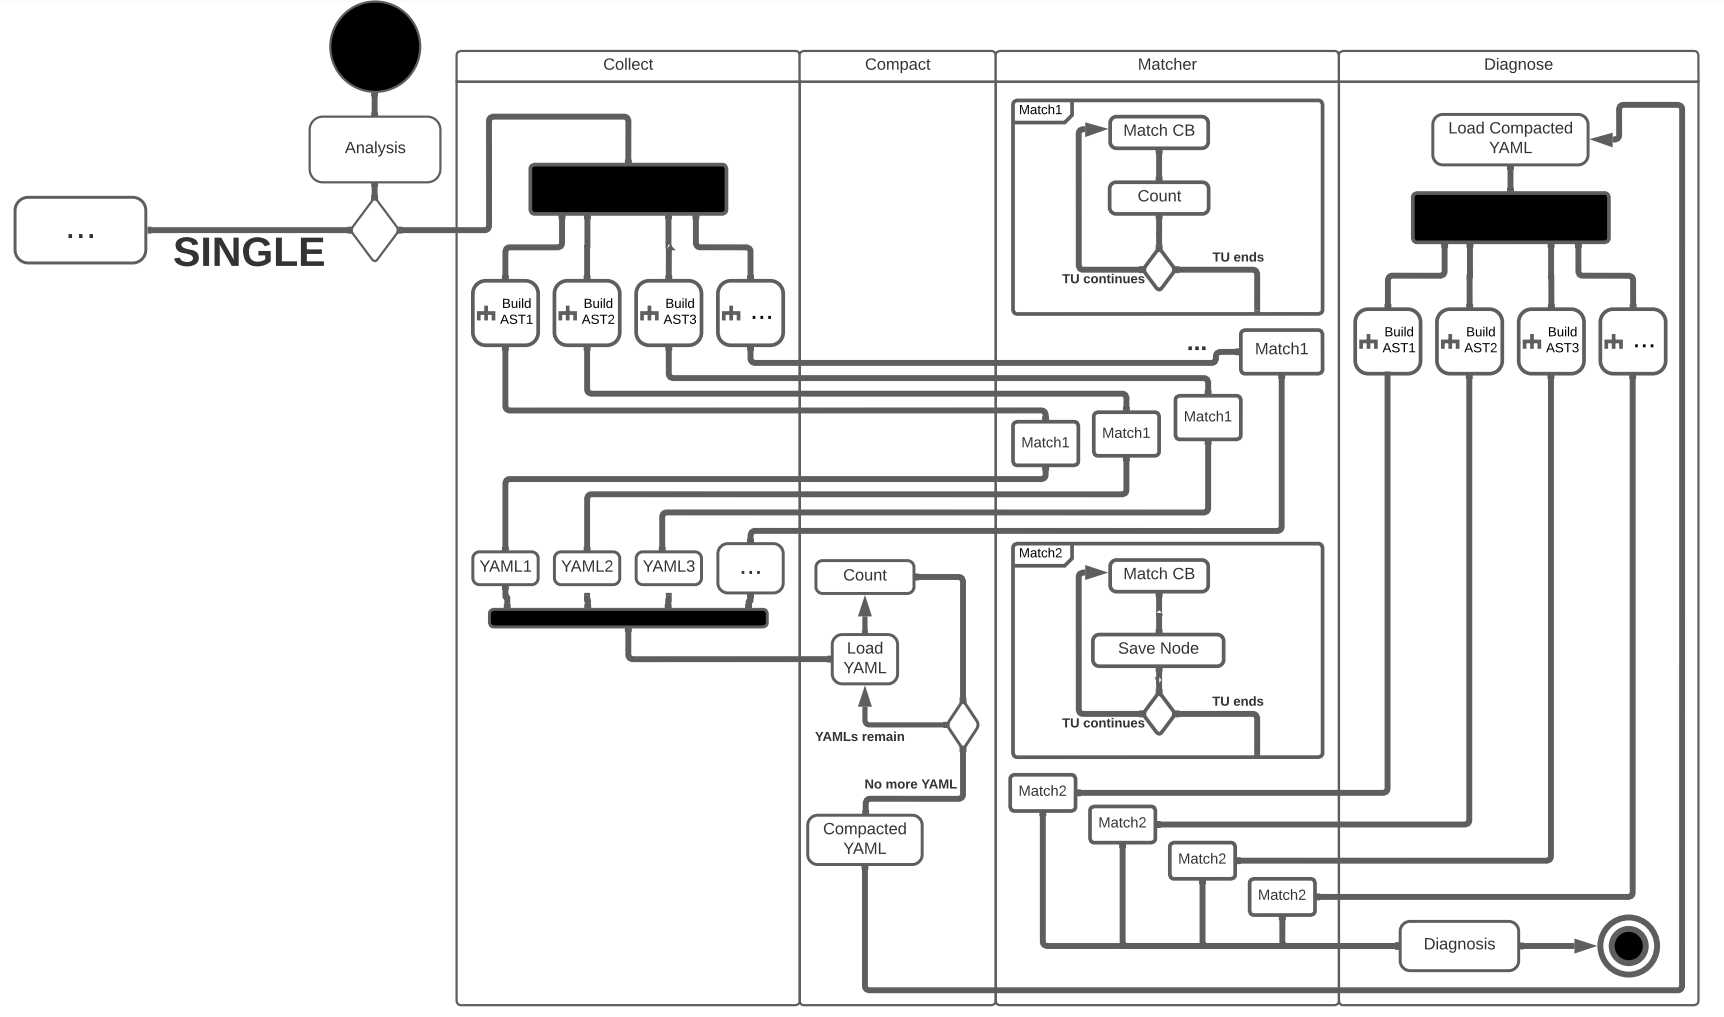
\includegraphics[width=\linewidth]{images/activity_multi.png}
	\caption{Activity diagram of Clang-Tidy infrastructure in "multi" mode.}
	\label{fig:activity-multi}
\end{figure}

The new flags I implemented are an \lstinline{enum} flag for the current phase that we are in, and a regular \lstinline{string}
for the collection directory path. If the directory does not currently extist on the given path, the infrastructure will create one.

The base class of the checkers, \texttt{ClangTidyCheck} already has \lstinline{virtual} functions for the checkers to override, with some
being optional and some not.
There are functions for \emph{\texttt{language support}}, registering \emph{\texttt{preprocessor callbacks}}, registering
\emph{\texttt{matchers}}, checking matched \emph{\texttt{AST nodes}}, and storing checker \emph{\texttt{options}}.
There are two additional functions from the base of
\texttt{ClangTidyCheck}, \texttt{MatchCallback}, and these are \texttt{onStartOfTranslationUnit and onEndOfTranslationUnit}, to
be able to do separate commands before and after the checker's actual work is done.

\begin{lstlisting}[language={C++},caption={Virtual functions from \texttt{ClangTidyCheck}'s header.},label={lst:ctc-single-virtual}]
/// Override this to register ``PPCallbacks`` in the preprocessor.
virtual void registerPPCallbacks(const SourceManager &SM,
  Preprocessor *PP,
  Preprocessor *ModuleExpanderPP) {}

/// Override this to register AST matchers with Finder.
virtual void registerMatchers(ast_matchers::MatchFinder *Finder) {}

/// ``ClangTidyChecks`` that register ASTMatchers should do the
/// actual work in here.
virtual void check(const ast_matchers::MatchFinder::MatchResult &Result) {}

/// Should store all options supported by this check with their
/// current values or default values for options that haven't been
/// overridden.
virtual void storeOptions(ClangTidyOptions::OptionMap &Options) {}
\end{lstlisting}

\begin{lstlisting}[language={C++},caption={Virtual functions from MatchCallback's header.},label={lst:mc-single-virtual}]
/// Called at the start of each translation unit.
/// Optionally override to do per translation unit tasks.
virtual void onStartOfTranslationUnit() {}

/// Called at the end of each translation unit.
/// Optionally override to do per translation unit tasks.
virtual void onEndOfTranslationUnit() {}
\end{lstlisting}

Originally, when a \emph{\texttt{callback}} happened (which we will address later in \cref{sec:dev-checker})
\texttt{ClangTidyChecker} simply called the derived \lstinline{class}'s \texttt{check} function.

\begin{lstlisting}[language={C++},caption={The old infrastructure's way of calling check.},label={lst:old-run}]
void ClangTidyCheck::run(const ast_matchers::MatchFinder::MatchResult &Result) {
	check(Result);
}
\end{lstlisting}

Now the checkers have three new \lstinline{virtual void} member functions to override: \texttt{collect}, \texttt{postCollect}
and \texttt{compact}.
It is important to note that this override is optional, in a sense, that some checkers can not be improved with and do not need
project-level knowledge. If one, however, decides to use the new multipass infrastructure with one's checker, then none of these overrides
are optional.
 
\texttt{ClangTidyChecker} has a private \texttt{ClangTidyContext} member called \texttt{Context}.
This contains information about the current phase, the directory path and the
phase \lstinline{enum} as well. This was used in the newly implemented member functions of the \texttt{ClangTidyChecker}
parent \lstinline{class}, and with protected getter functions, the derived checker can use some information from this context.


As we can see in \cref{lst:old-run}, this function only called the checker's \texttt{check}, but now it distinguishes two
out of our 3 separate
phases, diagnose and collect. In diagnose phase, it still calls for \texttt{check}, but in collect phase it calls
for the checker's separate \texttt{collect} function.

\begin{lstlisting}[language={C++},caption={Run function distinguishing Diagnose and Collect phase.},label={lst:new-run}]
void ClangTidyCheck::run(const ast_matchers::MatchFinder::MatchResult &Result) {
  switch (getPhase()) {
  case MultipassProjectPhase::Diagnose:
    check(Result);
    break;
  case MultipassProjectPhase::Collect:
    collect(Result);
    break;
  case MultipassProjectPhase::Compact:
    llvm_unreachable("AST Matchers should not have run in compact mode.");
  }
}
\end{lstlisting}

After the collection has been done on a translation unit, the destructor of the \lstinline{class} that
creates the checkers will call for the \texttt{runPostCollect} function of the base
\lstinline{class}, which as the name suggests, runs the \texttt{postCollect} function of the derived checker.

During compact phase, the infrastructure does not need the translation units at all, so there are no checkers instantiated during the
compilation, since this phase excludes compilation. Instead, the checker creation is now refactored into a function and that is called
in a separate path of the code, where we only create the checkers and call compact on each of them once.

In the following subsections I will explain how the \lstinline{virtual} functions should and how the member functions do work.

\subsection{Collect Function}

\texttt{collect} recieves the same parameters as check does, a \texttt{MatchResult} reference. In this function the checker should
do something similar to its original check function. Usually, it gets information out of the translation unit, and stores it in a data
structure of choise that is fit for the checker's logic.

\subsection{PostCollect Function}

\texttt{postCollect} recieves a \lstinline{StringRef}, the name of the output YAML file. In this function a checker should take all the data
collected from the translation unit, from the data structure, and write it in a YAML file whose filename is the function parameter.

\subsection{Compact Function}

\texttt{compact} has two parameters. One is a \lstinline{StringRef} that, similarly to \texttt{postCollect}, contains the
name of the output file.
The other is a \lstinline{vector<string>}s that contains all the YAML files in our multipass directory, that the
current checker created in the collect phase and wrote the collection data into for each translation unit.
In this phase, the checker should collect all the data from these YAML files and compact them into a single data structure. After
this step, it should write it into the YAML file whose filename is the function parameter.

\subsection{Additional Functions}

There are newly implemented protected functions to use aside from these \lstinline{virtual} ones:
\begin{itemize}
	\item \texttt{getCollectPath}: returns a \lstinline{string} to the path where the current check should write collected data to.
	\item \texttt{getCompactedDataPath}: returns a \lstinline{StringRef}, the name of the file where the current check should write or read compacted data to/from.
	\item \texttt{getPhase}: returns the \texttt{enum} representing the current phase
\end{itemize}

\section{Discarded Return Value Check} % külön a checker részek meg az infrat használórészek pls
\label{sec:dev-checker}

In \cref{sec:prob-state}, we justified the existence of a checker which focuses on detecting potential bugs and code smells
and giving warnings to function calls where the return value is ignored or unchecked, if we deem it necessary by analizing the ratio
of the amount of unchecked calls and all calls for the same function.

\subsection{Abstract Syntax Trees}

Before making a checker, first we should know about how checkers work. Clang-Tidy checkers perform pattern matching on
Clang's object oriented and strong typed representation of the abstract syntax tree of the source code.
ASTs represent the syntactic structure of a code as seen in \cref{fig:ast1}.

In \cref{fig:ast1} we have 2 function declarations, one of which is our main. We can see that our other function is called \texttt{foo},
that takes no parameters and returns an \lstinline{int}. In the \texttt{body} we have a statement, more specifically a
return statement. The subject of the return statement is a simple integer literal, with the value of 1.
In \texttt{main}, we only have another return statement, that has a call expression of a function that has a
declaration reference expression that refers to the declaration of our function \texttt{foo}.

Obviously, ASTs get increasingly more complex and harder to read as the source code grows. Another example can be seen on \cref{fig:ast2}.
\begin{figure}[H]
    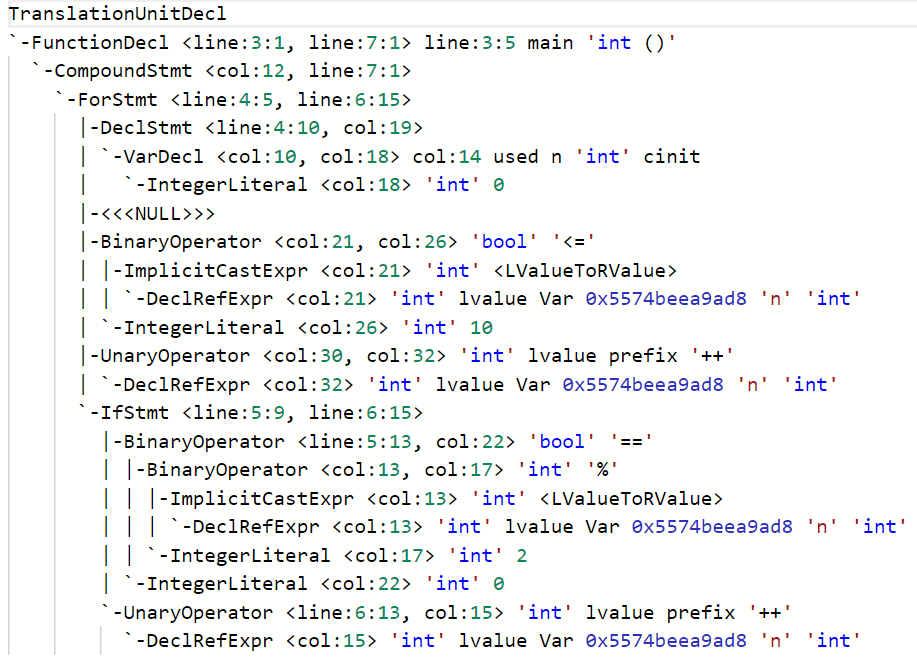
\includegraphics[width=\linewidth]{images/random_ast2.png}
	\caption{The AST of \cref{lst:ast2-code}}
    \label{fig:ast2}
\end{figure}

\begin{lstlisting}[language={C++},caption={The code of \cref{fig:ast2}.},label={lst:ast2-code}]
int main() {
	for (int n = 0; n <= 10; ++n)
		if (n % 2 == 0)
			++n;
}
\end{lstlisting}

\subsection{Pattern Matching}

Clang-Tidy checkers have \emph{\texttt{matchers}} that you can set up in the checker's overridden function \texttt{registerMatchers}.
This has its matcher, a \texttt{MatchFinder} as the parameter, and in this function we have to use its \texttt{addMatcher}
member function to add new patterns for it to match, and also to \texttt{bind} a string literal to the matches for later usage.
If the matcher finds a match, a \texttt{callback} action is executed.

In order to utilize the matches and the callbacks, we have to know how to match nodes on an AST. Clang-Tidy has built in matchers,
that we can see in the AST Matcher Reference~\cite{matcherref}. This tells us which matcher accepts which matcher or matchers as
parameter, and what their return type is. It also gives us examples of usage.
Theoretically, there are 3 distinct base types for AST nodes. \texttt{Decl} (declaration), \texttt{Stmt} (statement) and \texttt{Type}. In practice,
Clang-Tidy has more distinct bases in its AST representation, but for now let us view a a simple example of matching from
\texttt{Compiler Explorer}:\footnote{\url{https://godbolt.org/z/ncToe315q}, accessed 2022. 05. 14.}

\begin{lstlisting}[language={C++},caption={A very simple code for matching function calls.},label={lst:matchercode}]
int foo() { return 1; }

int main() {
	foo();
	int n = foo();
	return foo();
}
\end{lstlisting}

\begin{figure}[H]
    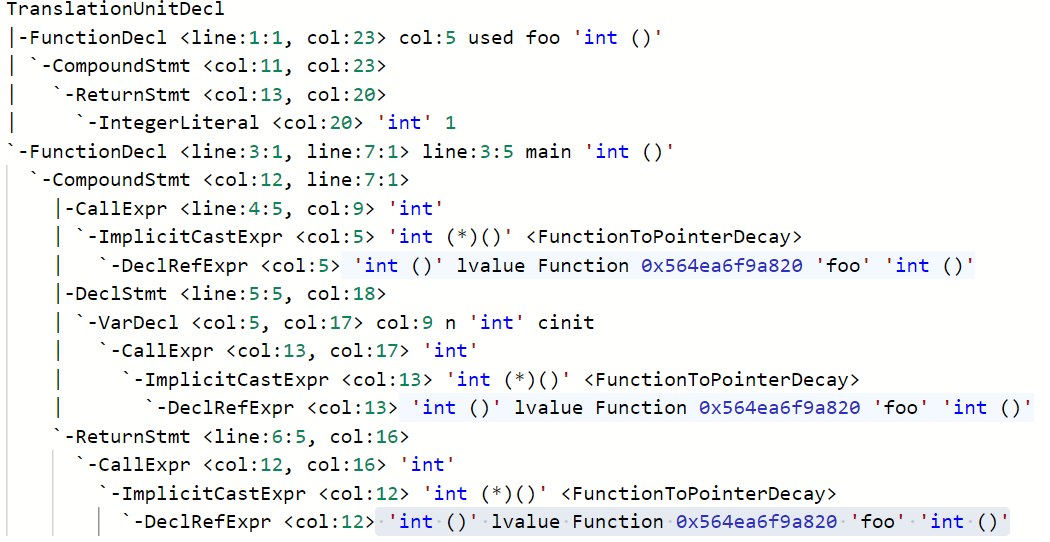
\includegraphics[width=\linewidth]{images/ast_for_matching.png}
	\caption{The AST of \cref{lst:matchercode}.}
    \label{fig:ast3}
\end{figure}

Here we can have 1 function declaration of the same function, and 3 call expressions, the first one in as a regular statement, the second one in
a variable declaration, and the third one in a return statement. Let us build a matcher for calls that a checker like mine should be
concerned about.
First, we want to match for function calls, whose declaration reference refers to a function declaration. If we use
\lstinline{match callExpr(callee(declRefExpr(to(functionDecl().bind("definition"))))).bind("call")} we get 3 matches
and 6 binds. It matches all 3 calls of \texttt{foo} bound to the literal \texttt{"call"}, and we also get 3 binds, all for the
first line, the \texttt{FunctionDecl} of \texttt{foo}, bound to \texttt{"definition"}.

We can also save the matcher bound to \texttt{"definition"} as a variable for easier usage and simplicity, if we wanted to.
With \lstinline{let Def functionDecl().bind("definition")} it will be saved as \texttt{Def}, and with
\lstinline{let Call callExpr(callee(declRefExpr(to(Def)))).bind("call")}, where we reuse our \texttt{Def}, we save our \texttt{Call} for later use. Now we only have
to match for \texttt{Call} with \lstinline{match Call} to get the same results.

We could improve it this matcher for the checker, with not matching functions declared with \lstinline{void} as return value.
In Clang-Tidy the "saved" matcher will be a
\lstinline{static const auto Call = callExpr(hasDeclaration(functionDecl(unless(returns(voidType())))));}. In reality, the
checker will need more specification in order to work properly, but this distinction is important as well.

There are separate matchers in static variables for any kind of usage of a return value, and then these are added in a single
\texttt{addMatcher} call of the matcher. Let us go through some of these matchers.

\subsubsection{Call}

Our actual specific call expression can be seen in \cref{lst:call}. Since this is the base of all other matchers
that we use, I will explain what we need to match for, in detail, starting with the bind. The \lstinline{static constexpr} that \texttt{Call}
is bound to is an \lstinline{llvm::StringLiteral} type, that wraps \texttt{"call"}.
We want to match for function calls, but not all function calls. First, we will sort out all functions whose declaration is a function
declaration to at least either a \lstinline{void} function, because they do not return a value to be checked or ignored, and a
function with \texttt{[[nodiscard]]}, since the compiler will already warn the user if needed. This is what we achive with lines
2-3. Second, we want to sort out any operator calls except for the following: \lstinline{()} or \lstinline{[]} operators
(this is done by lines 4-5), and \lstinline{*} or \lstinline{&} operators, but since those operators have multiple uses and
we want to include a specific use only, we only need these if they take only one arguement, also known as the \texttt{dereference}
and the \texttt{address-of} operator (which is achieved by lines 6-7).
All of this specification can be seen in \cref{fig:venn-call}.


\begin{lstlisting}[language={C++},caption={The matcher for our desired call expression.},label={lst:call}]
static const auto Call =
	callExpr(hasDeclaration(functionDecl(unless(anyOf(
				 returns(voidType()), hasAttr(attr::WarnUnusedResult))))),
			 unless(cxxOperatorCallExpr(
				 unless(anyOf(hasAnyOverloadedOperatorName("()", "[]"),
							  allOf(hasAnyOverloadedOperatorName("*", "&"),
									argumentCountIs(1)))))))
		.bind(::Call);
\end{lstlisting}

\begin{figure}[H]
	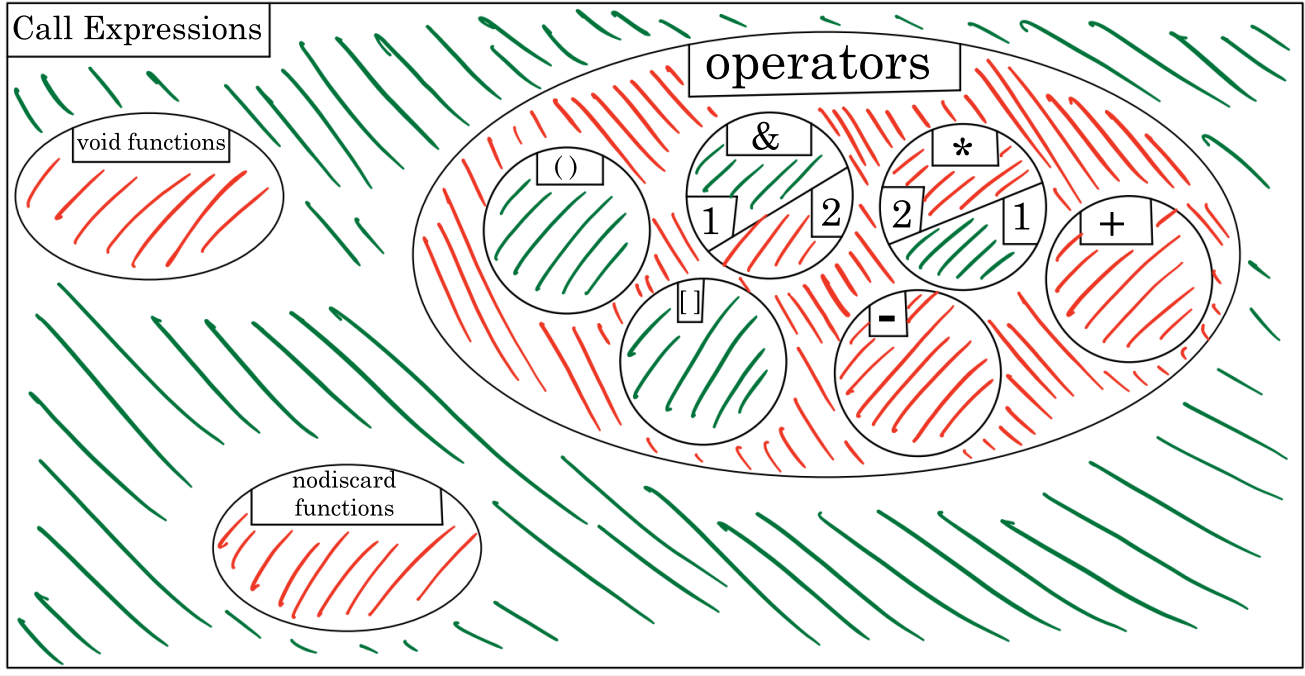
\includegraphics[width=\linewidth]{images/venn_call.png}
	\caption{A Venn-diagram of what \texttt{Call} matches, where 1 and 2 indicates arity. The green subsets are to be matched.}
	\label{fig:venn-call}
\end{figure}

\subsubsection{While}

In \cref{lst:while} we match
for either a \texttt{while} statement or a \texttt{do} statement that uses our call in their condition, and then since the matcher
\texttt{anyOf} does not automatically cast its return type to that of a statement, we do it manually with \texttt{stmt}.

\begin{lstlisting}[language={C++},caption={The matcher for usage in while expression.},label={lst:while}]
static const auto While =
	stmt(anyOf(whileStmt(hasCondition(Call)), doStmt(hasCondition(Call))));
\end{lstlisting}

\subsubsection{Return}

In \cref{lst:return} we simply match if a return statement uses our function as its return value.

\begin{lstlisting}[language={C++},caption={The matcher for the usage in return statement.},label={lst:return}] 
static const auto Return = returnStmt(hasReturnValue(Call));
\end{lstlisting} % TODO ide lehet törni kell a sort hogy ne legyen egyedül a caption az oldalon.

\subsubsection{For}

In \cref{lst:for} we match for
any and all of the following: if the \texttt{initialization}, the \texttt{condition}, or the \texttt{incrementation} of the for
loop, or if a \texttt{range-based} for loop, or any descendants of either of these uses the return value of our call.

\begin{lstlisting}[language={C++},caption={The matcher for the usage in for statement.},label={lst:for}]
static const auto For = anyOf(
	forStmt(eachOf(hasLoopInit(findAll(Call)), hasCondition(findAll(Call)),
				   hasIncrement(findAll(Call)))),
	cxxForRangeStmt(hasRangeInit(findAll(Call))));
\end{lstlisting}

We can also create new matchers, should we need one that is not yet in the library. % ezt majd whispy átnézi
It provides \emph{\texttt{macros}} that can be used to implement matchers with custom logic. For example in \cref{lst:hasassert} the
macro defines a single-parameter function called \texttt{hasAssertExpr} that takes a \texttt{Matcher<Expr>} called
\texttt{InnerMatcher} and returns a \texttt{Matcher<StaticAssertDecl>} object. It passes the
matcher into the assertion expression of assert, meaning if the inner matcher matches, the entire assertion will too.

\begin{lstlisting}[language={C++},caption={Custom logic and usage of a new matcher called \texttt{hasAssertExpr}.},label={lst:hasassert}]
AST_MATCHER_P(StaticAssertDecl, hasAssertExpr,
              ast_matchers::internal::Matcher<Expr>, InnerMatcher) {
  return InnerMatcher.matches(*Node.getAssertExpr(), Finder, Builder);
}

static const auto StaticAssert = staticAssertDecl(hasAssertExpr(Call));
\end{lstlisting}


\subsection{Checker Logic}

Before going into how my checker works, we should go through the member functions of it. The checker obviously overrides all
non-optional and some optional \lstinline{virtual} functions as seen in \cref{lst:override-header}. In \cref{lst:drv-member}
there are three additional member functions. These contain the logic of the checker and how it shapes
its data structure according to the current phase. 

\begin{lstlisting}[language={C++},caption={Overridden virtual functions in DiscardedReturnValueCheck's header.},label={lst:override-header}]
void registerMatchers(ast_matchers::MatchFinder *Finder) override;
void storeOptions(ClangTidyOptions::OptionMap &Opts) override;
void onStartOfTranslationUnit() override;
void onEndOfTranslationUnit() override;
void collect(const ast_matchers::MatchFinder::MatchResult &Result) override;
void postCollect(StringRef OutputFile) override;
void compact(const std::vector<std::string> &PerTuCollectedData,
			 StringRef OutputFile) override;
void check(const ast_matchers::MatchFinder::MatchResult &Result) override;
\end{lstlisting}

\begin{lstlisting}[language={C++},caption={Private member functions in DiscardedReturnValueCheck's header.},label={lst:drv-member}]
void matchResult(const ast_matchers::MatchFinder::MatchResult &Result,
                 bool ShouldCount);
void registerCall(const CallExpr *CE, const FunctionDecl *FD,
                  bool IncrementCounters, const void *ConsumingContext);
void diagnose(const Function &F);
\end{lstlisting}

For the data structure itself, The checker uses a \lstinline{struct} representing the functions with their tracked amount of calls and
checks (and its member function calculating the ratio of these in percentage), a \lstinline{StringMap} of functions to store their
name and their corresponding struct object, a \lstinline{DenseMap} of \lstinline{FunctionDecl - string} pairs, a
\lstinline{DenseMap} of \lstinline{CallExpr - SmallVector} pairs to prevent multiple callbacks on a single call expression
being processed the twice. It also uses a \lstinline{uint8_t} to save the the threshold option, and an \lstinline{Optional<bool>} to
track whether or not compacting has been done on the translation units.

\begin{lstlisting}[language={C++},caption={Members of the data structure.},label={lst:remaining-members}]
struct Function {
  std::size_t ConsumedCalls;
  std::size_t TotalCalls;
  const FunctionDecl *FD;
  llvm::SmallPtrSet<const CallExpr *, 32> DiscardedCEs;
  
  std::uint8_t ratio() const;
};
  using FunctionMapTy = llvm::StringMap<Function>;

  const std::uint8_t ConsumeThreshold;
  Optional<bool> CacheProjectDataLoadedSuccessfully;

  llvm::DenseMap<const CallExpr *, SmallVector<const void *, 2>> ConsumedCalls;
  llvm::DenseMap<const FunctionDecl *, std::string> FunctionIDs;
  FunctionMapTy CallMap;
\end{lstlisting}

After all the possible usages of a return value have been
refactored into these matchers, we put all of them into one call of \texttt{addMatcher} and bind them to
\texttt{"consume"}. In reality, the usages contain all 3 of the base node types, so we put these matchers into 3 \texttt{addMatcher} calls
in respect of which matcher returns which node type. The matchers \texttt{ExplicitCast, New, Delete, Argument, Unary, Dereference,
BinaryLHS, BinaryRHS, If, While, For, Switch, and Return} should return statements, \texttt{StaticAssert, VarDecl, and CtorInits}
should return declarations, and \texttt{Decltype, TemplateArg, and VLA} should return types.
Now all we have to do is match for a simple call.

\begin{lstlisting}[language={C++},caption={Separating the matchers to statement, declaration, and type.}]
  Finder->addMatcher(
	  traverse(
		  TK_IgnoreUnlessSpelledInSource,
		  stmt(eachOf(ExplicitCast, New, Delete, Argument, Unary, Dereference,
					  BinaryLHS, BinaryRHS, If, While, For, Switch, Return)))
		  .bind(Consume),
	  this);
  Finder->addMatcher(traverse(TK_IgnoreUnlessSpelledInSource,
							  decl(eachOf(StaticAssert, VarDecl, CtorInits)))
					     .bind(Consume),
				     this);
  Finder->addMatcher(traverse(TK_IgnoreUnlessSpelledInSource,
							  type(eachOf(Decltype, TemplateArg, VLA)))
					     .bind(Consume),
				     this);

  Finder->addMatcher(traverse(TK_IgnoreUnlessSpelledInSource, Call), this);
\end{lstlisting}

The checker will match for all function calls (that are not declared \lstinline{void} et cetera) bound to \texttt{"call"}, and for the ones
that are checked it will match once more with the bind \texttt{"consume"}. For every match the callback happens and since matching \texttt{"consume"}
deterministically comes before matching \texttt{"call"}, we can be sure that if we matched with \texttt{"consume"} it is a checked call, and if we did
not, it is an unchecked call so we can count the checks of our matched call expressions accordingly. In \cref{lst:consume} we try to
get our \texttt{"consume"} bound node for either of the 3 base node types, and if either gets a node back, we count it as a checked return.
Otherwise we count it as unchecked.

\begin{lstlisting}[language={C++},caption={Catching nodes of used return values.},label={lst:consume}]
void DiscardedReturnValueCheck::matchResult(
	const MatchFinder::MatchResult &Result, bool ShouldCount) {
  const auto *CE = Result.Nodes.getNodeAs<CallExpr>(Call);
  assert(CE && "Bad matcher");

  const void *ConsumeNode = nullptr;
  if (const auto *D = Result.Nodes.getNodeAs<Decl>(Consume))
    ConsumeNode = D;
  if (const auto *S = Result.Nodes.getNodeAs<Stmt>(Consume))
    ConsumeNode = S;
  if (const auto *T = Result.Nodes.getNodeAs<Type>(Consume))
    ConsumeNode = T;
  if (ConsumeNode)
    return registerCall(CE, CE->getDirectCallee(), ShouldCount, ConsumeNode);
  if (ConsumedCalls.find(CE) == ConsumedCalls.end())
	return registerCall(CE, CE->getDirectCallee(), ShouldCount, nullptr);
}
\end{lstlisting}

Then the call expression is emplaced in our data structure for counting and because we do not want to count the same call twice, and if
the call belongs to a function declaration that have previously been saved in our data structure, then we also increment its data in
respect of it being checked or not.

At the end of the translation unit, we give our diagnostics.

\subsection{Multipass phases}

It is very clear that a checker like this is almost completely useless for projects larger than a single translation unit, unless we use
the enhanced infrastructure. This makes the checker a perfect fit to test it. First, we have to implement the new \lstinline{virtual} functions.

\texttt{collect} does the same thing as the old \texttt{check} callback did. Because of this, the logic of this step was put
into a member function and is called in both functions, \texttt{check} and \texttt{collect}.

We save declarations and adjust the data structure with each new call of the same function. At the end of a translation unit, \texttt{postCollect}
writes this data into a new YAML file under the unique name that was generated by the infrastructure.

\texttt{compact} reads in all the data from the collection files, fills up the data structure and then it writes the compacted data into the output YAML.
Because both writing and reading into our data structure is necessary more than once in the checker, this also have been refactored, and \texttt{compact},
\texttt{postCollect} and \texttt{check} all call these functions.

In \cref{lst:load}, we can see that we first extract the data from the YAML file into an optional \lstinline{vector} of the function representation,
and if the extraction actually happened, we emplace and modify the data of the files into the current state of the data structure. At the end, it returns
whether succesful extraction happened or not.
In \cref{lst:write} we see that \texttt{writeYAML} puts our data into the output \texttt{stream}.
These are both examples of possible writing and loading methods for YAML serialization that are easy to use and implement using LLVM's YAML library~\cite{yamllib}.

\begin{lstlisting}[language={C++},caption={Functions for loading.},label={lst:load}]
using FunctionVec = std::vector<SerializedFunction>;

static Optional<FunctionVec> loadYAML(StringRef File) {
  using namespace llvm;
  
  ErrorOr<std::unique_ptr<MemoryBuffer>> IStream =
  	MemoryBuffer::getFileAsStream(File);
  if (!IStream)
    return None;
  
  FunctionVec R;
  yaml::Input YIn{**IStream};
  YIn >> R;
  
  return R;
}
  
static bool loadYAML(StringRef FromFile,
					   DiscardedReturnValueCheck::FunctionMapTy &ToMap) {
  Optional<FunctionVec> OV = loadYAML(FromFile);
  if (!OV)
    return false;
  
  for (const SerializedFunction &SF : *OV) {
    DiscardedReturnValueCheck::Function &F =
      ToMap
    	  .try_emplace(SF.ID,
    				   DiscardedReturnValueCheck::Function{0, 0, nullptr, {}})
    	  .first->second;
    
    F.ConsumedCalls += SF.ConsumedCalls;
    F.TotalCalls += SF.TotalCalls;
  }
  
  return true;
}
\end{lstlisting}

\begin{lstlisting}[language={C++},caption={Function for writing.},label={lst:write}]
static void writeYAML(StringRef Whence, FunctionVec Elements,
                      StringRef ToFile) {
  std::error_code EC;
  llvm::raw_fd_ostream FS(ToFile, EC, llvm::sys::fs::OF_Text);
  if (EC) {
    llvm::errs() << "DiscardedReturnValueCheck: Failed to write " << Whence
                 << " output file: " << EC.message();
    llvm::report_fatal_error("", false);
    return;
  }

  llvm::yaml::Output YAMLOut(FS);
  YAMLOut << Elements;
}
\end{lstlisting}

Both \texttt{postCollect} and \texttt{compact} uses \texttt{writeYAML} with the YAML compatible representation of the function representation. For the
purpose of writing, these functions both use a refactored function that converts the latter into the YAML compatible version. These are seen in
\cref{lst:yamlize} with the method of making a \lstinline{struct} YAML compatible as well.

\begin{lstlisting}[language={C++},caption={Steps for making the data YAML writable.},label={lst:yamlize}]
struct SerializedFunction {
  std::string ID;
  std::size_t ConsumedCalls, TotalCalls;
};

template <> struct MappingTraits<SerializedFunction> {
  static void mapping(IO &IO, SerializedFunction &F) {
    IO.mapRequired("ID", F.ID);
    IO.mapRequired("Consumed", F.ConsumedCalls);
    IO.mapRequired("Total", F.TotalCalls);
  }
};

LLVM_YAML_IS_SEQUENCE_VECTOR(SerializedFunction)

static FunctionVec
yamlize(const DiscardedReturnValueCheck::FunctionMapTy &Map) {
  FunctionVec SFs;
  llvm::transform(Map, std::back_inserter(SFs), [](auto &&E) {
    return SerializedFunction{E.first().str(), E.second.ConsumedCalls,
                              E.second.TotalCalls};
  });
  return SFs;
}
\end{lstlisting}

Check works in a similar way. First, we check if compact has happened already. If not, check runs without project-level knowledge and emits diagnostics
per translation unit, the same
way as before. If compact phase has not been run for this cheker, we fill up our data structure, but only if this step has not happened before.
For this, we use the same refactored functions as in \texttt{collect}, \texttt{matchResult} and thus \texttt{registerCalls}, with the exception
that adjustments in the data structure after each call does not need to happen, since all the data on the amount of checks and calls had been acquired before,
from the compacted file. Then we take the unique name (as a \lstinline{string}) of a function
declaration, or generate one if one does not already exist. After this we check again, whether or not we stored this declaration in the data structure,
and if not, we store it, but only if its call was unused, and then if compact has not happened, we increment its data accordingly. If it
has, we have nothing left to do. Now we only need to emit diagnostics to the right calls, which happens at the end of each translation unit.

\section{Evaluation}
\label{sec:eval}

This checker's upgrade to the multipass infrastructure differs from the original one only by a little. However,
it gives us very different results. The checker has run on large projects. It ran with 50\% and 80\% threshold both with and
without collection and compacting. The results are shown in \cref{tab:proj-test}
\pagebreak
%\begin{center}
	\begin{longtable}{ | m{0.35\textwidth} | m{0.2\textwidth} | m{0.14\textwidth} | m{0.18\textwidth} | } % jobbra a számok és ezres , \,
		
		\hline
		\textbf{Project name} & \textbf{Multi-pass?} & \textbf{Threshold} & \textbf{\# reports}  \\
		\hline \hline
		\endfirsthead
		
		\hline
		\textbf{Project name} & \textbf{Multi-pass?} & \textbf{Threshold} & \textbf{\# reports}  \\
		\hline \hline
		\endhead

		\hline
		\endfoot
		\endlastfoot

		\multirow{4}{*}{Bitcoin \texttt{v0.20.1}~\cite{bitcoin}}
		& \ding{53} & \hfill{}50\% & \hfill{}140 \\
		& \ding{51} & \hfill{}50\% & \hfill{}320 \\
		& \ding{53} & \hfill{}80\% & \hfill{}25 \\
		& \ding{51} & \hfill{}80\% & \hfill{}92 \\
		\hline

		\multirow{4}{*}{CodeChecker \texttt{v6.17.0}~\cite{codechecker}}
		& \ding{53} & \hfill{}50\% & \hfill{}2 \\
		& \ding{51} & \hfill{}50\% & \hfill{}5 \\
		& \ding{53} & \hfill{}80\% & \hfill{}0 \\
		 & \ding{51} & \hfill{}80\% & \hfill{}0 \\
		\hline

		\multirow{4}{*}{Contour \texttt{v0.2.0.173}~\cite{contour}}
		& \ding{53} & \hfill{}50\% & \hfill{}38 \\
		& \ding{51} & \hfill{}50\% & \hfill{}107 \\
		& \ding{53} & \hfill{}80\% & \hfill{}10 \\
		 & \ding{51} & \hfill{}80\% & \hfill{}8 \\
		\hline

		\multirow{4}{*}{cURL \texttt{7.66.0}~\cite{curl}}
		& \ding{53} & \hfill{}50\% & \hfill{}55 \\
		& \ding{51} & \hfill{}50\% & \hfill{}210 \\
		& \ding{53} & \hfill{}80\% & \hfill{}6 \\
		 & \ding{51} & \hfill{}80\% & \hfill{}104 \\
		\hline

		\multirow{4}{*}{FFmpeg \texttt{n4.3.1}~\cite{ffmpeg}}
		& \ding{53} & \hfill{}50\% & \hfill{}904 \\
		& \ding{51} & \hfill{}50\% & \hfill{}1\,846 \\
		& \ding{53} & \hfill{}80\% & \hfill{}148 \\
		 & \ding{51} & \hfill{}80\% & \hfill{}613 \\
		 \hline 

		 \multirow{4}{*}{libWebM \texttt{1.0.0.27}~\cite{libwebm}}
		 & \ding{53} & \hfill{}50\% & \hfill{}9 \\
		 & \ding{51} & \hfill{}50\% & \hfill{}10 \\
		 & \ding{53} & \hfill{}80\% & \hfill{}0 \\
		 & \ding{51} & \hfill{}80\% & \hfill{}1 \\
		 \hline 
		 
		 \multirow{4}{*}{LLVM \texttt{12.0.0}~\cite{llvm}}
		 & \ding{53} & \hfill{}50\% & \hfill{}4\,615 \\
		 & \ding{51} & \hfill{}50\% & \hfill{}6\,837 \\
		 & \ding{53} & \hfill{}80\% & \hfill{}1\,077 \\
		  & \ding{51} & \hfill{}80\% & \hfill{}2\,150 \\
		 \hline

		 \multirow{4}{*}{Memcached \texttt{1.6.8}~\cite{memcached}}
		 & \ding{53} & \hfill{}50\% & \hfill{}32 \\
		 & \ding{51} & \hfill{}50\% & \hfill{}49 \\
		 & \ding{53} & \hfill{}80\% & \hfill{}5 \\
		  & \ding{51} & \hfill{}80\% & \hfill{}16 \\
		 \hline

		 \multirow{4}{*}{MongoDB \texttt{r4.4.6}~\cite{mongo}}
		 & \ding{53} & \hfill{}50\% & \hfill{}1\,671 \\
		 & \ding{51} & \hfill{}50\% & \hfill{}2\,463 \\
		 & \ding{53} & \hfill{}80\% & \hfill{}370 \\
		  & \ding{51} & \hfill{}80\% & \hfill{}1\,223 \\
		  \hline 

		 \multirow{4}{*}{OpenSSL \texttt{3.0.0}~\cite{openssl}}
		 & \ding{53} & \hfill{}50\% & \hfill{}427 \\
		 & \ding{51} & \hfill{}50\% & \hfill{}1\,060 \\
		 & \ding{53} & \hfill{}80\% & \hfill{}56 \\
		  & \ding{51} & \hfill{}80\% & \hfill{}244 \\
		 \hline 

		\multirow{4}{*}{PostgreSQL \texttt{r13.0}~\cite{postgres}}
		& \ding{53} & \hfill{}50\% & \hfill{}799 \\
		& \ding{51} & \hfill{}50\% & \hfill{}644 \\
		& \ding{53} & \hfill{}80\% & \hfill{}62 \\
		 & \ding{51} & \hfill{}80\% & \hfill{}215 \\
		\hline 

		\multirow{4}{*}{Protocol Buffers \texttt{v3.13.0}~\cite{protobuf}}
		& \ding{53} & \hfill{}50\% & \hfill{}51 \\
		& \ding{51} & \hfill{}50\% & \hfill{}122 \\
		& \ding{53} & \hfill{}80\% & \hfill{}20 \\
		 & \ding{51} & \hfill{}80\% & \hfill{}75 \\
		\hline 

		\multirow{4}{*}{Qt Base \texttt{v6.2.0}~\cite{qtbase}}
		& \ding{53} & \hfill{}50\% & \hfill{}1\,195 \\
		& \ding{51} & \hfill{}50\% & \hfill{}2\,764 \\
		& \ding{53} & \hfill{}80\% & \hfill{}200 \\
		 & \ding{51} & \hfill{}80\% & \hfill{}1\,093 \\
		\hline
		
		\multirow{4}{*}{SQLite \texttt{3.33.0}~\cite{sqlite}}
		& \ding{53} & \hfill{}50\% & \hfill{}284 \\
		& \ding{51} & \hfill{}50\% & \hfill{}288 \\
		& \ding{53} & \hfill{}80\% & \hfill{}42 \\
		 & \ding{51} & \hfill{}80\% & \hfill{}48 \\
		\hline
		
		\multirow{4}{*}{tmux \texttt{2.6}~\cite{tmux}}
		& \ding{53} & \hfill{}50\% & \hfill{}35 \\
		& \ding{51} & \hfill{}50\% & \hfill{}48 \\
		& \ding{53} & \hfill{}80\% & \hfill{}1 \\
		 & \ding{51} & \hfill{}80\% & \hfill{}1 \\
		\hline
		
		\multirow{4}{*}{twin \texttt{v0.8.1}~\cite{twin}}
		& \ding{53} & \hfill{}50\% & \hfill{}54 \\
		& \ding{51} & \hfill{}50\% & \hfill{}69 \\
		& \ding{53} & \hfill{}80\% & \hfill{}9 \\
		 & \ding{51} & \hfill{}80\% & \hfill{}22 \\
		\hline
		
		\multirow{4}{*}{Vim \texttt{v8.2.1920}~\cite{vim}}
		& \ding{53} & \hfill{}50\% & \hfill{}227 \\
		& \ding{51} & \hfill{}50\% & \hfill{}383 \\
		& \ding{53} & \hfill{}80\% & \hfill{}32 \\
		 & \ding{51} & \hfill{}80\% & \hfill{}54 \\
		\hline
		
		\multirow{4}{*}{Xerces \texttt{v3.2.3}~\cite{xerces}}
		& \ding{53} & \hfill{}50\% & \hfill{}125 \\
		& \ding{51} & \hfill{}50\% & \hfill{}197 \\
		& \ding{53} & \hfill{}80\% & \hfill{}9 \\
		 & \ding{51} & \hfill{}80\% & \hfill{}38 \\
		\hline
		
		\caption{Results of different runs on live projects.} \label{tab:proj-test}
	\end{longtable}
%\end{center}

In \cref{tab:proj-test}, we can see that the numbers between both single and multiple phase, and 50\% and 80\% threshold runs largely differ
in a considerable amount of test projects. There were results where the multiple phase run gave more warnings, indicating the aforementioned
bugs hiding in separate translation units only, and some results where it gave less warnings, indicating false positives in single runs.

In \cref{fig:ff-80-single} and \cref{fig:ff-80-multi}, we can see diagrams of the results. Each line represents a function, with
its height as the total amount of calls. The green and red parts represent the checked and unchecked calls, respectively. The descending graph of black
dots display the ratio of checked to all calls, which is important regarding our threshold.

In these runs, the amount of separate unchecked functions were similar, but using the multi-pass infrastructure, the amount of calls for these functions was
obviously a lot higher. In the old infrastructure run, the ratios are closer to the 80\% threshold, and most functions here were called less than 20
times, and were only unchecked once or twice. However, if we look at the multi-pass run, the ratios are a lot higher. They were unchecked only
a couple of times in this run as well, but the amount of total calls per function was bigger than in the previous run, resulting in the
functions staying more consistently above our 80\% threshold.

\begin{figure}[H]
	\makebox[\textwidth]{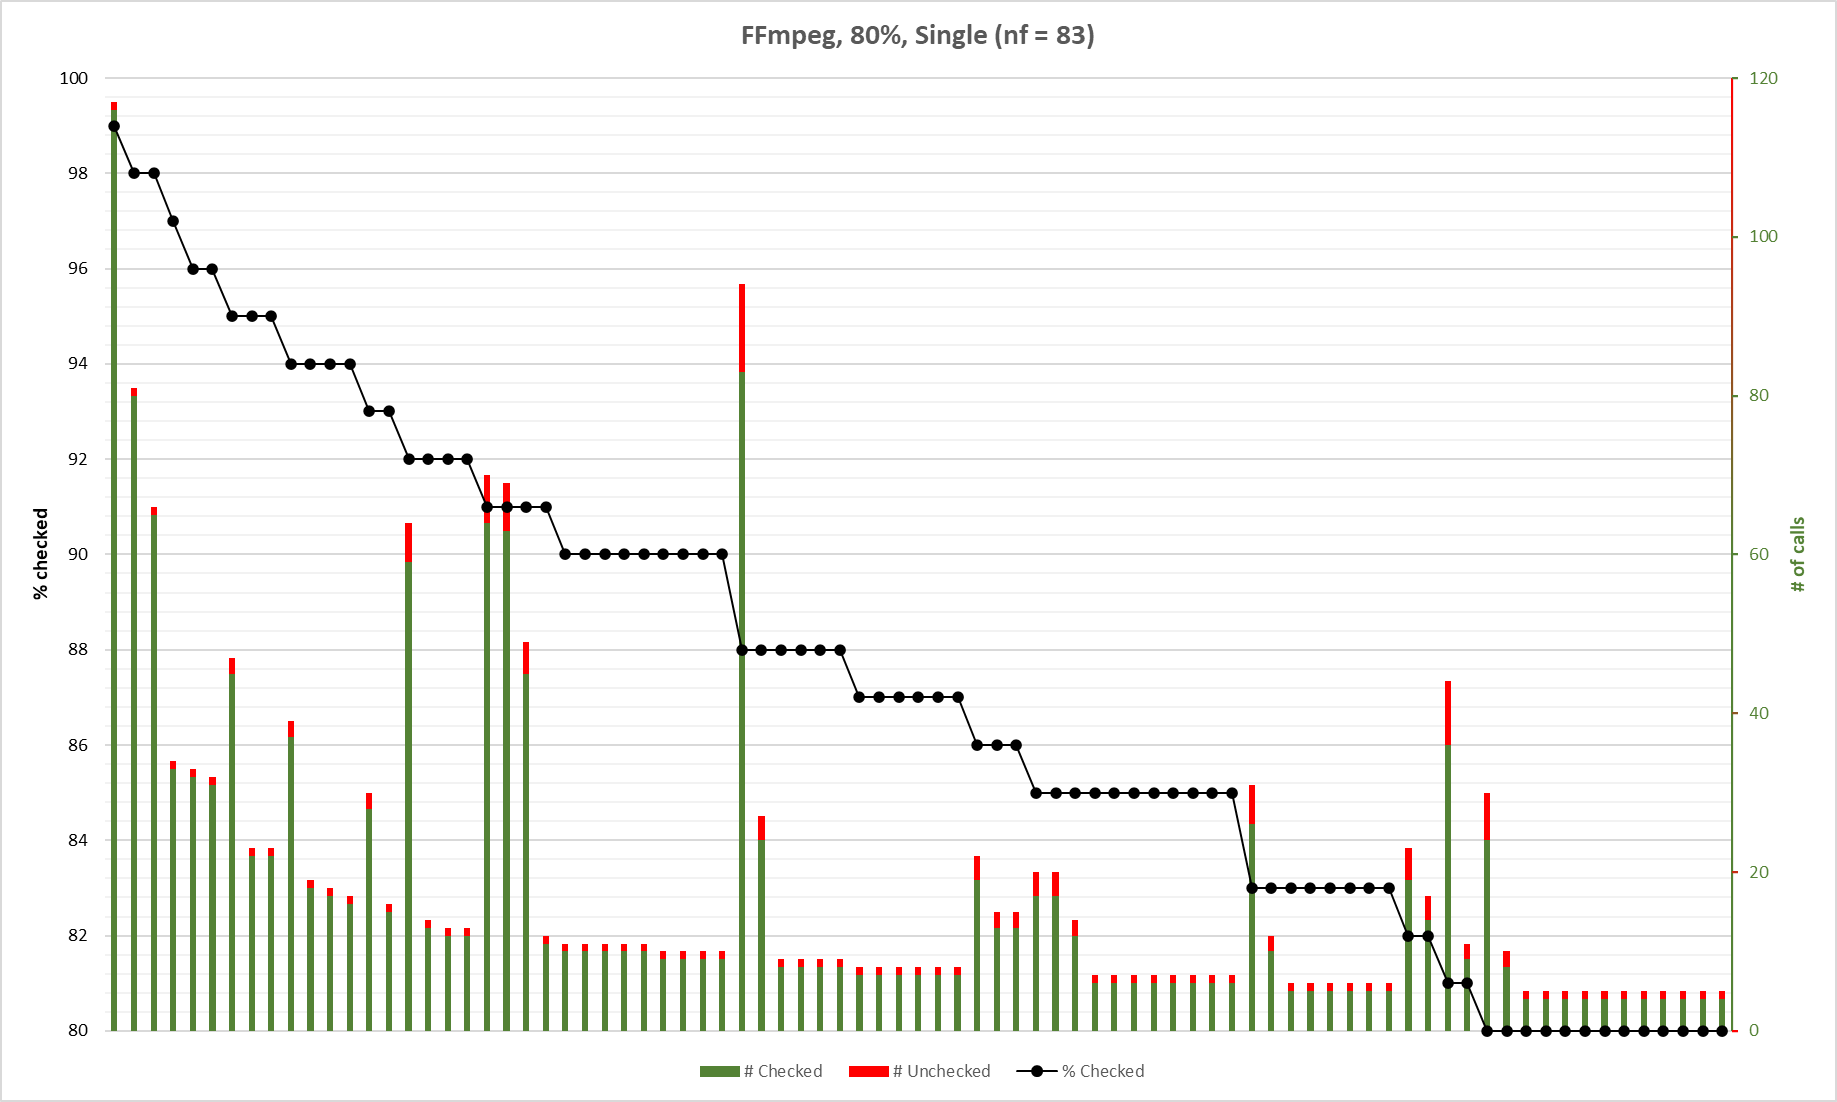
\includegraphics[width=1.2\linewidth]{images/FFmpeg_80_1_Single.png}}
	\caption{Diagram of 80\% threshold single run on FFmpeg.}
	\label{fig:ff-80-single}
\end{figure}

\begin{figure}[H]
	\makebox[\textwidth]{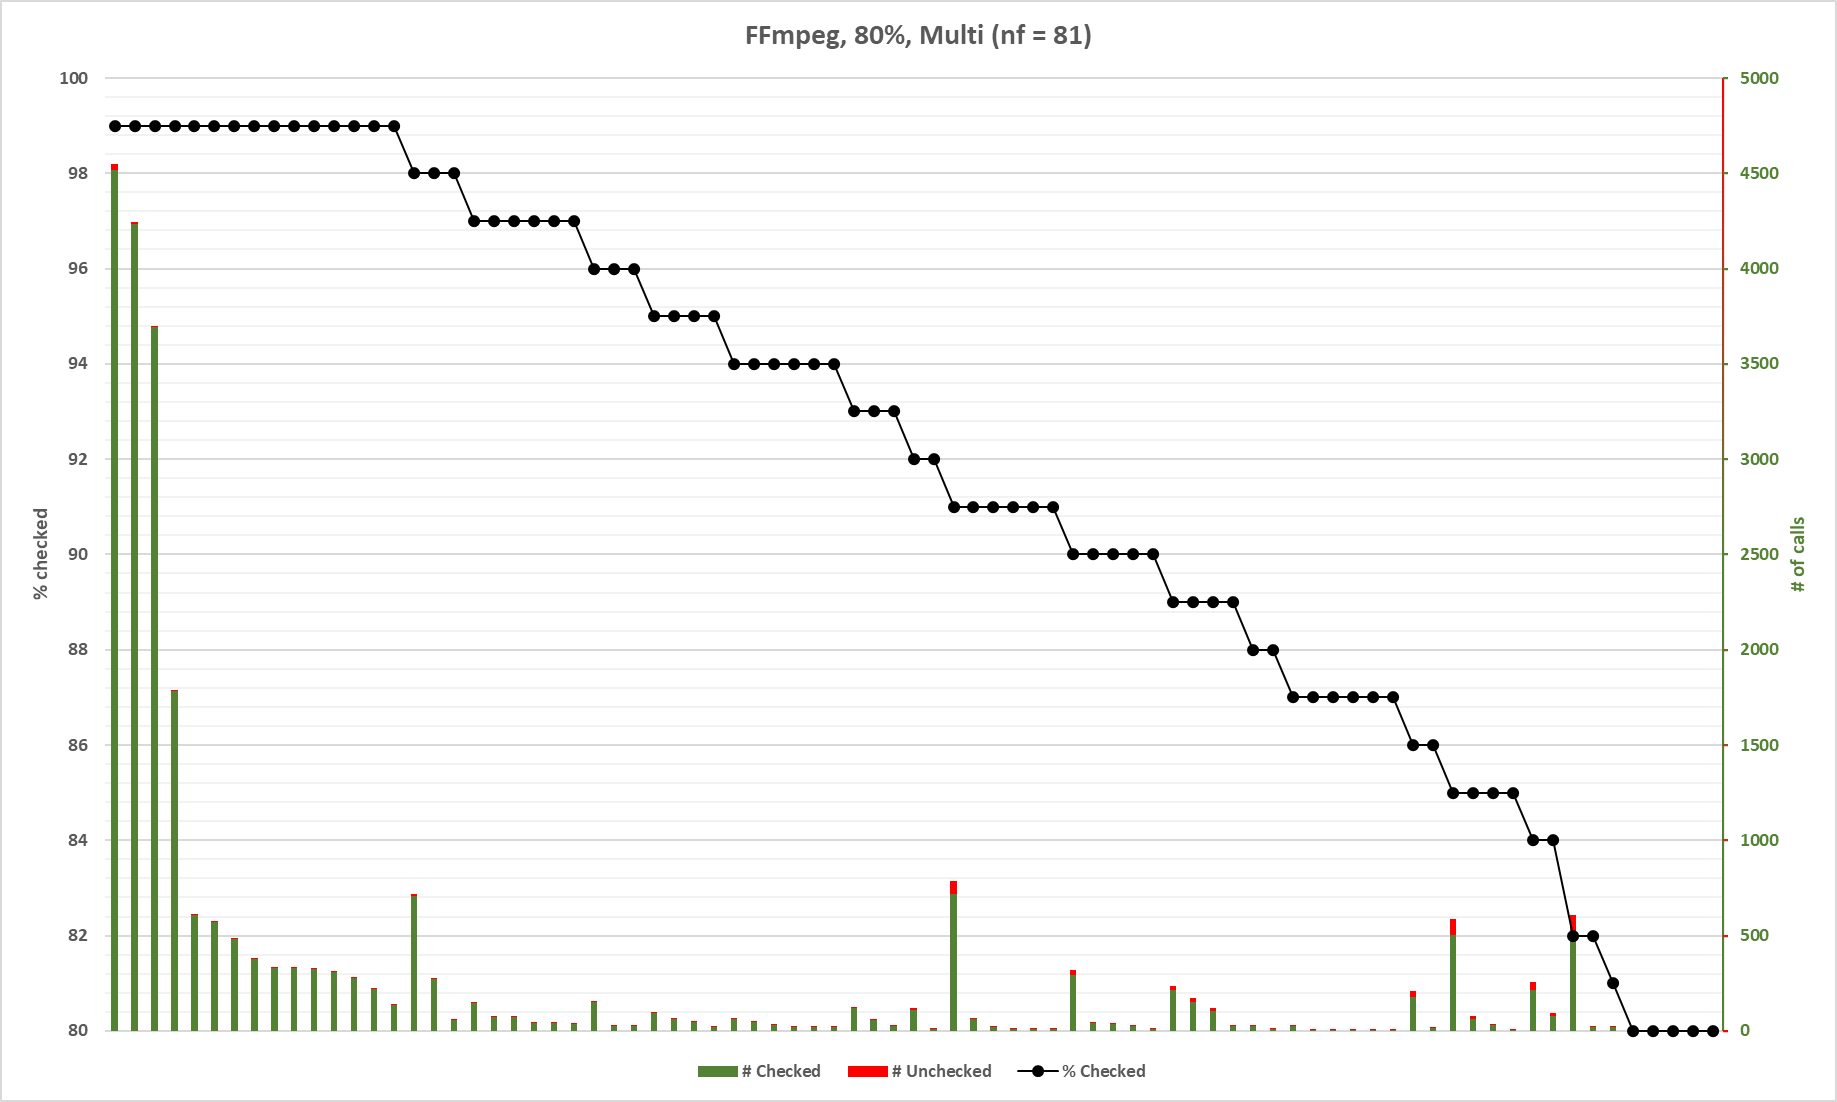
\includegraphics[width=1.2\linewidth]{images/FFmpeg_80_2_Multi.png}}
	\caption{Diagram of 80\% threshold multi run on FFmpeg.}
	\label{fig:ff-80-multi}
\end{figure}

Let us take a look at a 50\% threshold run comparison as well. In \cref{fig:bc-50-single} and \cref{fig:bc-50-multi} we get very different
results again. Here we can still see the higher ratios in the multi run, as well as higher overall amount of function calls. This time we
have more unchecked calls for functions that have been called considerably more than the rest, in both amount and ratio.

\begin{figure}[H]
	\makebox[\textwidth][c]{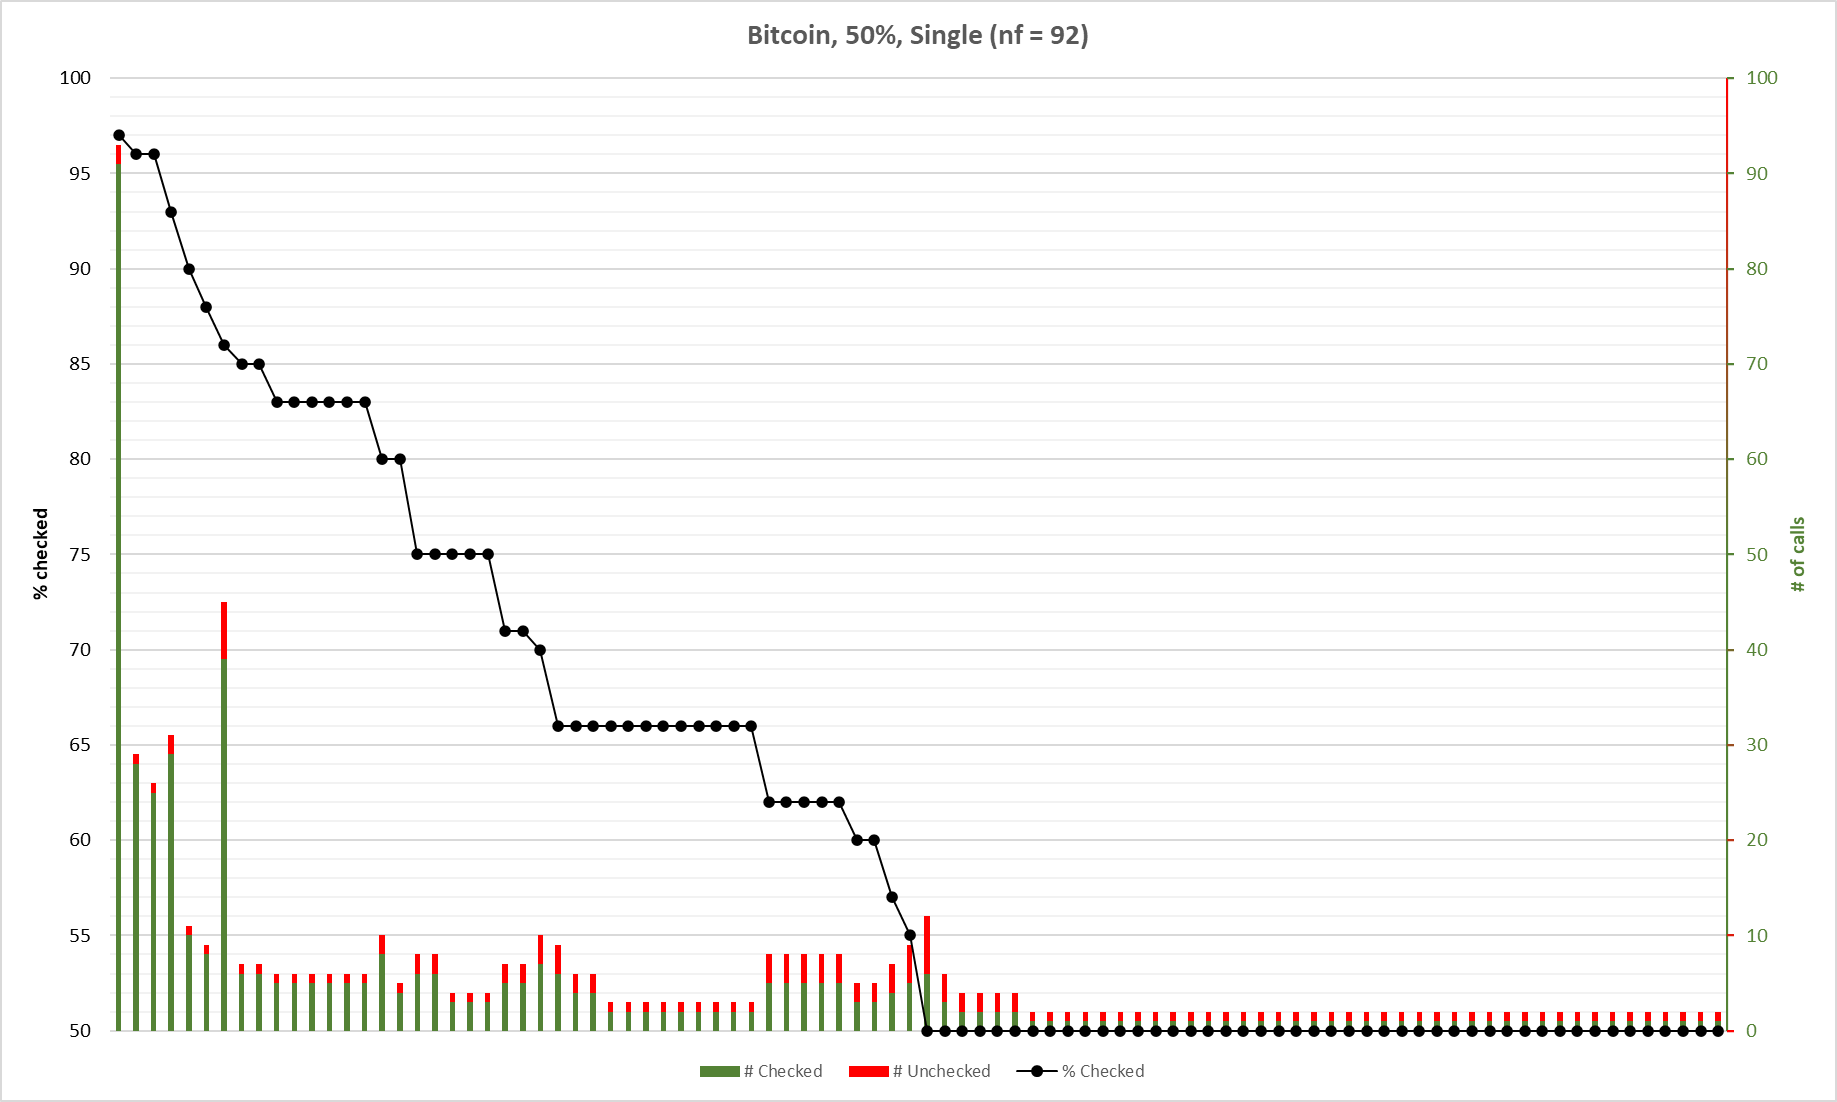
\includegraphics[width=1.2\linewidth]{images/Bitcoin_50_1_Single.png}}
	\caption{Diagram of 50\% threshold single run on Bitcoin.}
	\label{fig:bc-50-single}
\end{figure}

\begin{figure}[H]
	\makebox[\textwidth][c]{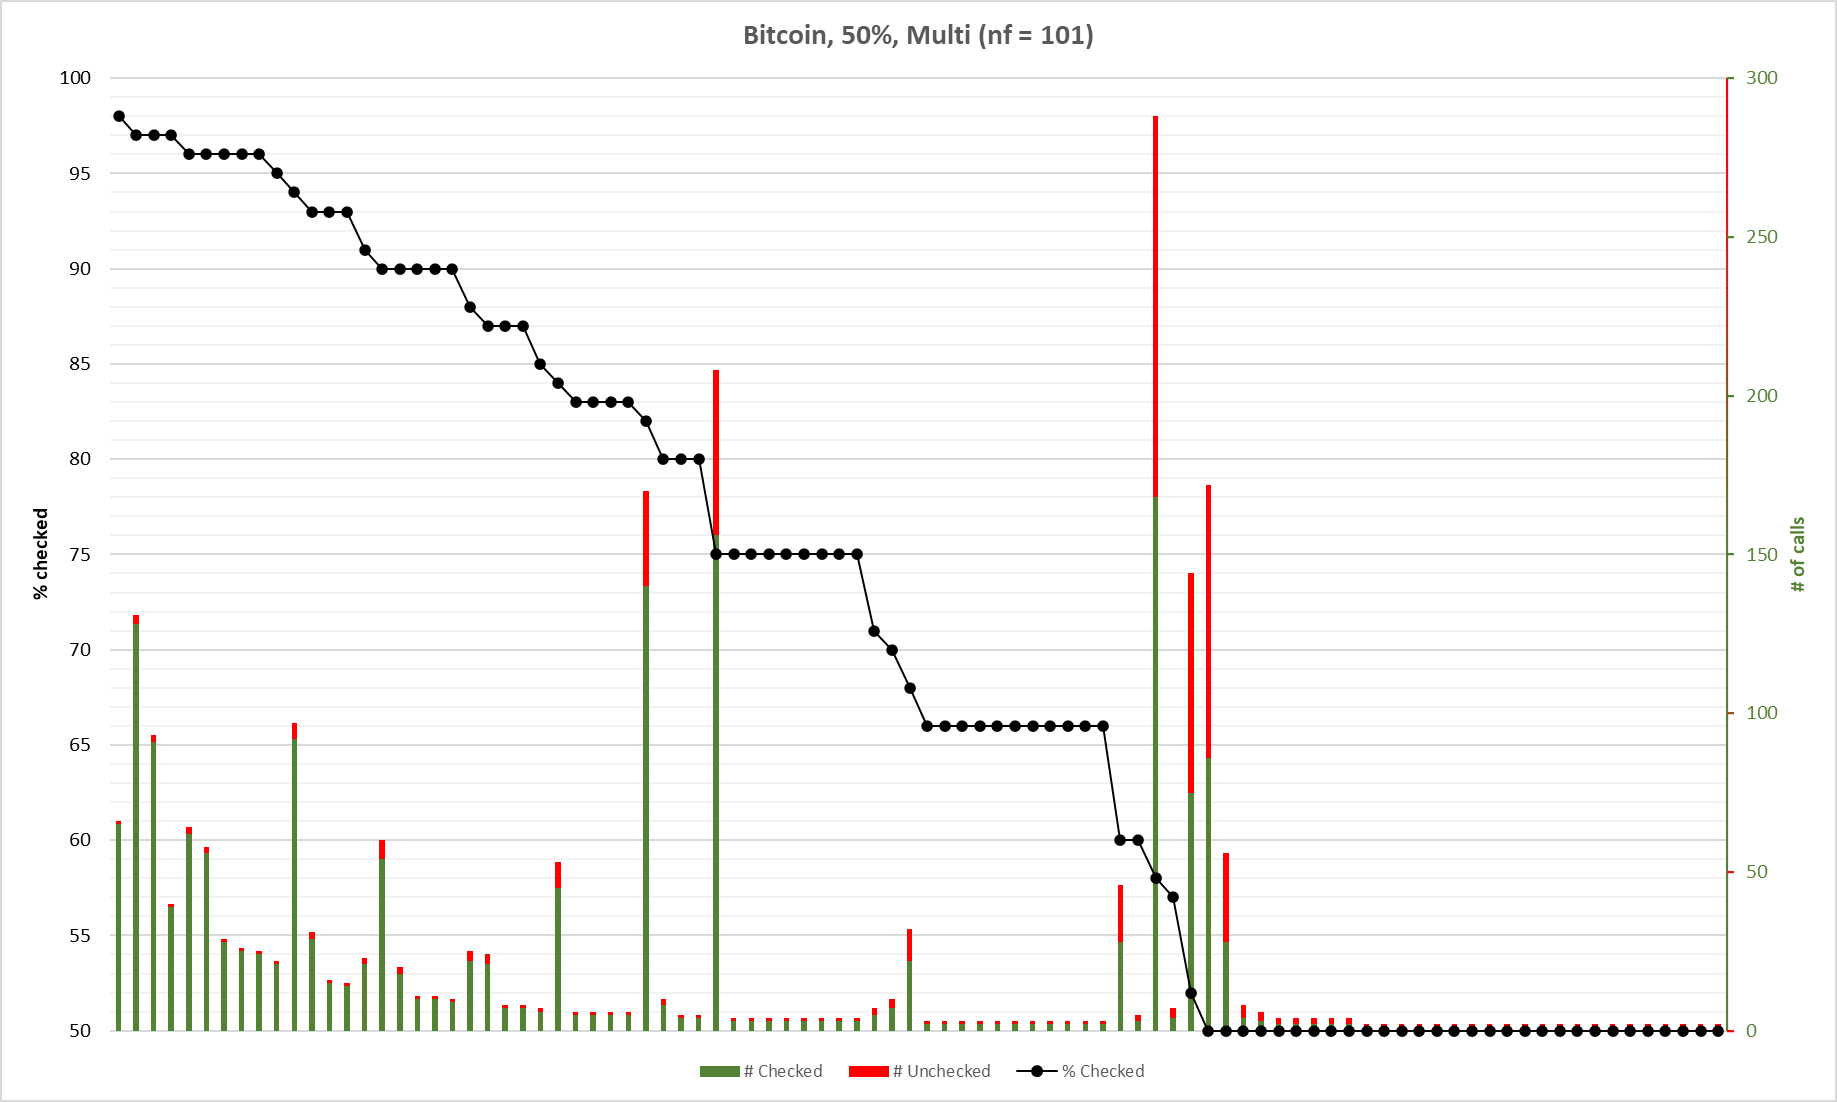
\includegraphics[width=1.2\linewidth]{images/Bitcoin_50_2_Multi.png}}
	\caption{Diagram of 50\% threshold multi run on Bitcoin.}
	\label{fig:bc-50-multi}
\end{figure}

The diagrams for all of the aforementioned project tests can be found in \cref{appx:diagrams}.
What can be said about almost all of the larger results is that they have a great amount of functions barely passing the threshold whose total
amount of calls do not exceed a considerable number compared to the size of the project and some other functions within the results. These could
potentially be ignored in some cases in the future.











\iffalse
\chapter{hide2}

\begin{lstlisting}[language={C++},caption={},label={}]

\end{lstlisting}


Lorem ipsum dolor sit amet, consectetur adipiscing elit. Duis nibh leo, dapibus in elementum nec, aliquet id sem. Suspendisse potenti.
 Nullam sit amet consectetur nibh. Donec scelerisque varius turpis at tincidunt.

\section{Theorem-like environments}

\begin{definition}
Mauris tristique sollicitudin ultrices. Etiam tristique quam sit amet metus dictum imperdiet. Nunc id lorem sed nisl pulvinar aliquet 
vitae quis arcu. Morbi iaculis eleifend porttitor.
\end{definition}

Maecenas rutrum eros sem, pharetra interdum nulla porttitor sit amet. In vitae viverra ante. Maecenas sit amet placerat orci, sed tinc
idunt velit. Vivamus mattis, enim vel suscipit elementum, quam odio venenatis elit, et mollis nulla nunc a risus. Praesent purus m
agna, tristique sed lacus sit amet, convallis malesuada magna. Phasellus faucibus varius purus, nec tristique enim porta vitae.

\begin{theorem}
Nulla finibus ante vel arcu tincidunt, ut consectetur ligula finibus. Mauris mollis lectus sed ipsum bibendum, ac ultrices erat dictum
. Suspendisse faucibus euismod lacinia. Etiam vel odio ante.
\end{theorem}
\begin{proof}
Etiam pulvinar nibh quis massa auctor congue. Pellentesque quis odio vitae sapien molestie vestibulum sit amet et quam. Pellentesque v
el dui eget enim hendrerit finibus at sit amet libero. Quisque sollicitudin ultrices enim, nec porta magna imperdiet vitae. Cras c
ondimentum nunc dui.
\end{proof}

Donec dapibus sodales ante, at scelerisque nunc laoreet sit amet. Mauris porttitor tincidunt neque, vel ullamcorper neque pulvinar et.
 Integer eu lorem euismod, faucibus lectus sed, accumsan felis. 

\begin{remark}
Nunc ornare mi at augue vulputate, eu venenatis magna mollis. Nunc sed posuere dui, et varius nulla. Sed mollis nibh augue, eget scele
risque eros ornare nec. Praesent porta, metus eget eleifend consequat, eros ligula eleifend ex, a pellentesque mi est vitae urna. 
Vivamus turpis nunc, iaculis non leo eget, mattis vulputate tellus.
\end{remark}

Fusce in aliquet neque, in pretium sem. Donec tincidunt tellus id lectus pretium fringilla. Nunc faucibus, erat pretium tempus tempor,
 tortor mi fringilla neque, ac congue ex dui vitae mauris. Donec pretium et quam a cursus.

\begin{note}
Aliquam vehicula luctus mi a pretium. Nulla quam neque, maximus nec velit in, aliquam mollis tortor. Aliquam erat volutpat. Curabitur 
vitae laoreet turpis. Integer id diam ligula.
\end{note}

Ut sollicitudin tempus urna et mollis. Aliquam et aliquam turpis, sed fermentum mauris. Nulla eget ex diam. Donec eget tellus pharetra
, semper neque eget, rutrum diam.

\subsection{Equations, formulas}

Duis suscipit ipsum nec urna blandit, $2 + 2 = 4$ pellentesque vehicula quam fringilla. Vivamus euismod, lectus sit amet euismod viver
ra, dolor metus consequat sapien, ut hendrerit nisl nulla id nisi. Nam in leo eu quam sollicitudin semper a quis velit.

$$a^2 + b^2 = c^2$$

Phasellus mollis, elit sed convallis feugiat, dolor quam dapibus nibh, suscipit consectetur lacus risus quis sem. Vivamus scelerisque 
porta odio, vitae euismod dolor accumsan ut.

In mathematica, identitatem Euleri (equation est scriptor vti etiam notum) sit aequalitatem Equation~\ref{eq:euler}:
\begin{equation}\label{eq:euler}
e^{i \times \pi} + 1 = 0
\end{equation}


\section{Source code samples}

Nulla sodales purus id mi consequat, eu venenatis odio pharetra. Cras a arcu quam. Suspendisse augue risus, pulvinar a turpis et, 
commodo aliquet turpis. Nulla aliquam scelerisque mi eget pharetra. Mauris sed posuere elit, ac lobortis metus. Proin lacinia sit
amet diam sed auctor. Nam viverra orci id sapien sollicitudin, a aliquam lacus suscipit. Quisque ac tincidunt leo Code~\ref{src:cpp}
and \ref{src:csharp}:

\lstset{caption={Hello World in C++}, label=src:cpp}
\begin{lstlisting}[language={C++}]
#include <stdio>

int main() 
{
	int c;
	std::cout << "Hello World!" << std::endl;

	std::cout << "Press any key to exit." << std::endl;
	std::cin >> c;
	
	return 0;
}
\end{lstlisting}

\lstset{caption={Hello World in C\#}, label=src:csharp}
\begin{lstlisting}[language={[Sharp]C}]
using System;
namespace HelloWorld
{
	class Hello 
	{
		static void Main() 
		{
			Console.WriteLine("Hello World!");
			
			Console.WriteLine("Press any key to exit.");
			Console.ReadKey();
		}
	}
}
\end{lstlisting}

\subsection{Algorithms}

A general Interval Branch and Bound algorithm is shown in Algorithm~\ref{alg:ibb}. An appropriate selection rule is applied
in Step~\ref{step:selrule}.\\
Source of example: \href{https://www.inf.u-szeged.hu/actacybernetica/}{Acta Cybernetica (this is a hyperlink)}.

\begin{algorithm}[H]
\caption{A general interval B\&B algorithm} 
\label{alg:ibb} 
\textbf{\underline{Funct}} IBB($S,f$)
\begin{algorithmic}[1] % display line numbers before every n line, here n = 1
\State Set the working list ${\cal L}_W$ := $\{S\}$ and the final list ${\cal L}_Q$ := $\{\}$     
\While{( ${\cal L}_W \neq \emptyset$ )} \label{alg:igoend}
	\State  Select an interval $X$ from ${\cal L}_W$ \label{step:selrule}\Comment{Selection rule}  
	\State Compute $lbf(X)$ \Comment{Bounding rule}		  
	\If{$X$ cannot be eliminated} \Comment{Elimination rule}
		\State Divide $X$ into $X^j,\ j=1,\dots, p$, subintervals   \Comment{Division rule}
		\For{$j=1,\ldots,p$}
			\If{$X^j$ satisfies the termination criterion} \Comment{Termination rule}
				\State Store $X^j$ in ${\cal L}_W$ 
			\Else
				\State Store $X^j$ in ${\cal L}_W$ 
			\EndIf
		\EndFor  
	\EndIf
\EndWhile
\State \textbf{return} ${\cal L}_Q$
\end{algorithmic}
\end{algorithm}
\fi